\begin{center}
    \begin{figure}[H]
        \centering

        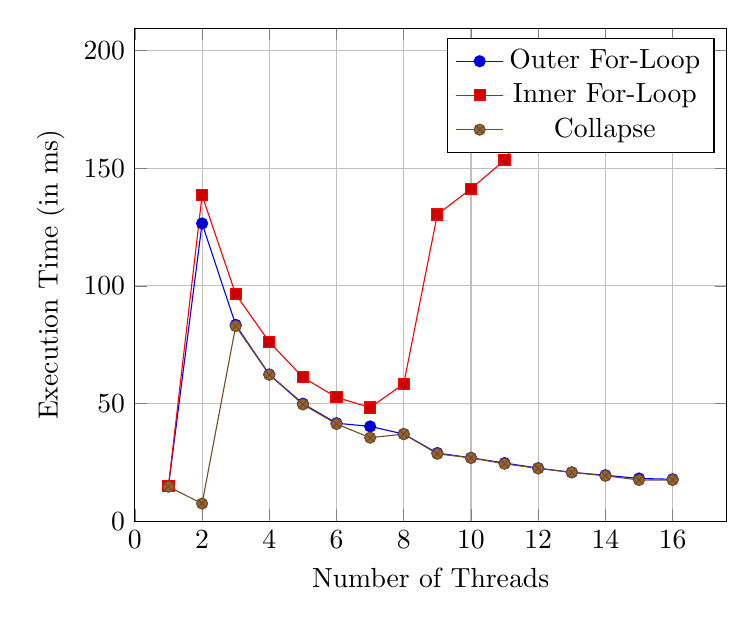
\begin{tikzpicture}
            \begin{axis}[
                title={},
                width=0.75\textwidth,
                xlabel={Number of Threads},
                ylabel={Execution Time (in ms)},
                xmin=0,
                ymin=0,
                grid=major
            ]
                \addplot coordinates {
                    (1,14.8915)(2,126.488)(3,83.4241)(4,62.3742)(5,49.9608)(6,41.6626)(7,40.2989)(8,37.0454)(9,28.9892)(10,26.956)(11,24.7474)(12,22.5727)(13,20.7843)(14,19.574)(15,18.1935)(16,17.8497)
                };
                \addlegendentry{Outer For-Loop}

                \addplot coordinates {
                    (1,15.1484)(2,138.43)(3,96.4194)(4,76.1557)(5,61.1348)(6,52.636)(7,48.3067)(8,58.3773)(9,130.291)(10,141.226)(11,153.341)(12,177.499)(13,189.672)(14,170.349)(15,167.978)(16,190.359)
                };
                \addlegendentry{Inner For-Loop}       

                \addplot coordinates {
                    (1,14.6987)(2,7.53125)(3,82.8959)(4,62.2286)(5,49.6344)(6,41.3342)(7,35.5147)(8,37.0327)(9,28.6662)(10,26.9202)(11,24.4288)(12,22.4487)(13,20.7811)(14,19.3091)(15,17.5392)(16,17.5417)
                };
                \addlegendentry{Collapse}
            \end{axis}
        \end{tikzpicture}
        \caption{Grayscale Performance Tests dice.png}
    \end{figure}
\end{center}